\documentclass[aspectratio=169,11pt]{beamer}
\usepackage[T1]{fontenc}
\usepackage{lmodern,amsmath,booktabs,graphicx}
\definecolor{Ink}{HTML}{223047}
\definecolor{Blue}{HTML}{2166AC}
\definecolor{Orange}{HTML}{D47720}
\setbeamercolor{normal text}{fg=Ink,bg=white}
\setbeamercolor{frametitle}{fg=Ink}
\setbeamercolor{structure}{fg=Blue}
\setbeamerfont{frametitle}{size=\LARGE,series=\bfseries}
\setbeamertemplate{navigation symbols}{}
\setbeamertemplate{frametitle}{\vspace{.35cm}\insertframetitle\par}
\setbeamertemplate{footline}{\hfill\scriptsize\color{Ink!60}\insertframenumber\hspace{.6cm}\vspace{.3cm}}
\setbeamersize{text margin left=.7cm,text margin right=.7cm}
\newcommand{\source}[1]{\par\vfill{\tiny\color{Ink!65}#1}}
\newcommand{\luxburg}{\href{https://www.tml.cs.uni-tuebingen.de/teaching/2024_statistical_learning/downloads_free/vorlesung_main.pdf}{U. von Luxburg, Statistical Machine Learning (2024)}}
\begin{document}

\begin{frame}{A threshold splits both score distributions}
Predict positive when the model score $s\geq t$.
\begin{columns}[c]
\begin{column}{.66\textwidth}
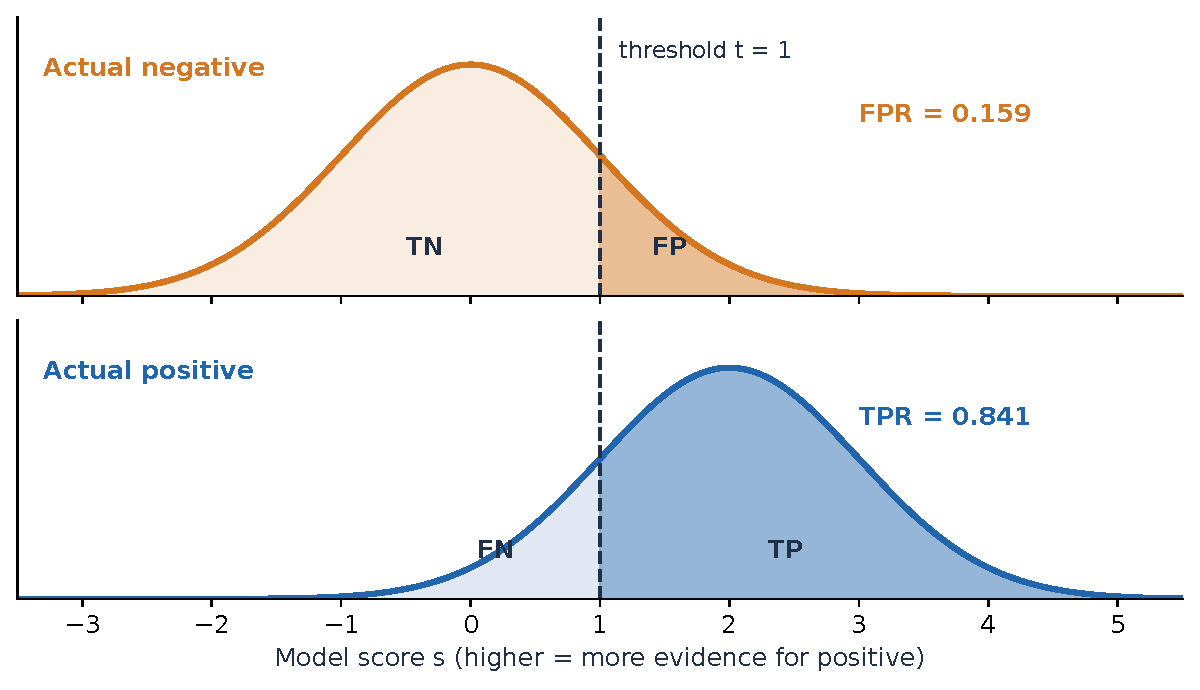
\includegraphics[width=\linewidth]{figures/distributions.pdf}
\end{column}
\begin{column}{.32\textwidth}
\textbf{Positive if $s\geq t$}
\smallskip

\textcolor{Blue}{True positive rate}
\[\mathrm{TPR}=\frac{\mathrm{TP}}{\mathrm{TP}+\mathrm{FN}}\]
\textcolor{Orange}{False positive rate}
\[\mathrm{FPR}=\frac{\mathrm{FP}}{\mathrm{FP}+\mathrm{TN}}\]
\small Lower $t$: more true and false positives.
\end{column}
\end{columns}
\source{TP/TN: true positives/negatives. FP/FN: false positives/negatives. Each density has area 1.\\Intuition inspired by \luxburg. Own illustrative Gaussian plots.}
\end{frame}

\begin{frame}{The ROC curve collects all decision thresholds}
\begin{columns}[c]
\begin{column}{.52\textwidth}
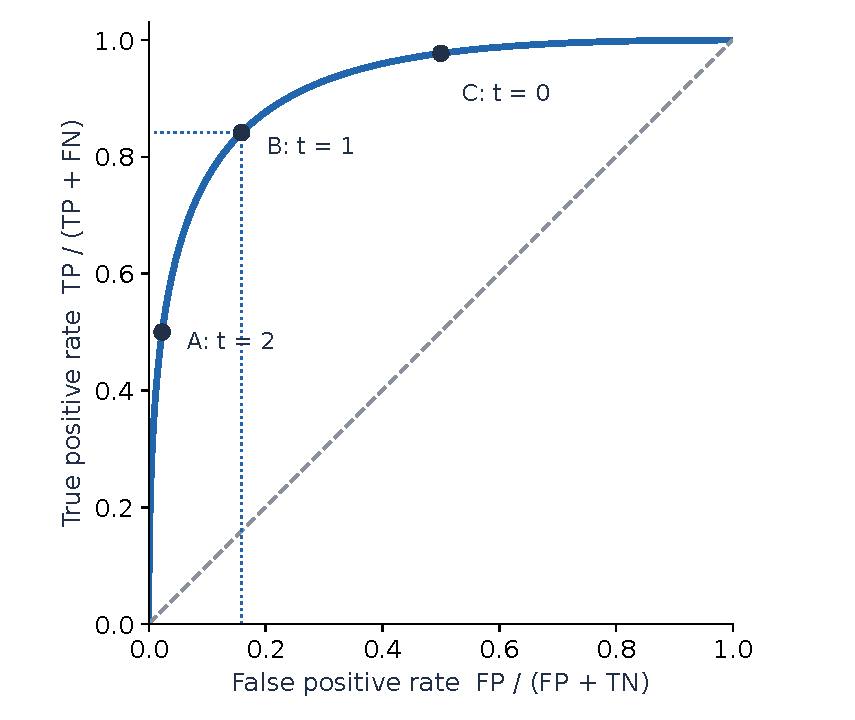
\includegraphics[width=.94\linewidth]{figures/roc.pdf}
\end{column}
\begin{column}{.45\textwidth}
\small\textbf{Receiver Operating Characteristic}
\smallskip

Each threshold gives one point\[\bigl(\mathrm{FPR}(t),\mathrm{TPR}(t)\bigr).\]
\centering
\small\renewcommand{\arraystretch}{1.25}
\begin{tabular}{lrrr}
&$t$&FPR&TPR\\\midrule
A&2&0.023&0.500\\
B&1&0.159&0.841\\
C&0&0.500&0.977\\\bottomrule
\end{tabular}
\par\raggedright\small\smallskip
Sweep $t$ from $+\infty$ to $-\infty$:\\
$(0,0)$: nobody positive.\\
$(1,1)$: everybody positive.
\smallskip

Upper left: high TPR, low FPR.
\end{column}
\end{columns}
\source{Own illustrative curve. ROC definition: \luxburg;\\\href{https://scikit-learn.org/stable/modules/generated/sklearn.metrics.roc_curve.html}{scikit-learn, roc\_curve}. Finite datasets give discrete operating points.}
\end{frame}

\begin{frame}{AUC summarizes ranking across thresholds}
\begin{columns}[c]
\begin{column}{.51\textwidth}
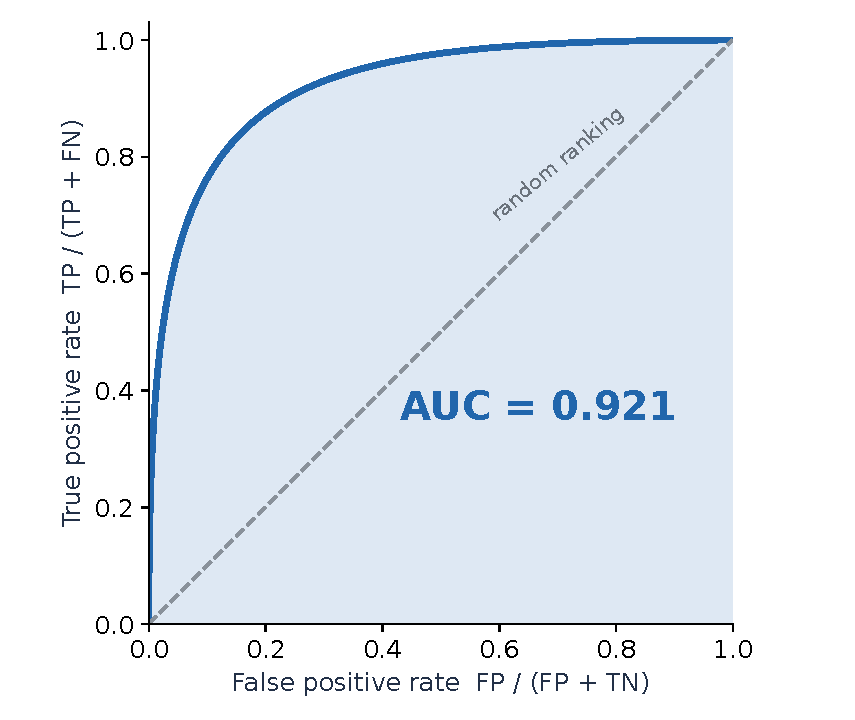
\includegraphics[width=.94\linewidth]{figures/auc.pdf}
\end{column}
\begin{column}{.46\textwidth}
\small\textbf{Area under the ROC curve}
\[\mathrm{AUC}=\int_0^1\mathrm{TPR}(u)\,du\]
\small Here $u$ denotes the false positive rate.
\smallskip

\textbf{Ranking intuition}
\smallskip

How often does a random positive score higher than a random negative?
\smallskip

\textbf{1.0}: perfect ranking.\\
\textbf{0.5}: random-ranking reference.
\smallskip

\small AUC $=0.8$: the positive wins 80\% of pairs (assuming no ties). This does not mean 80\% accuracy.
\end{column}
\end{columns}
\source{Ties count as half a win. AUC does not choose a threshold. Own illustrative curve.\\Sources: \href{https://doi.org/10.1016/j.patrec.2005.10.010}{T. Fawcett (2006), An introduction to ROC analysis}; \href{https://scikit-learn.org/stable/modules/generated/sklearn.metrics.roc_auc_score.html}{scikit-learn, roc\_auc\_score}.}
\end{frame}
\end{document}
